\chapter{Convolutional Neural Networks (CNNs)}
\label{Chapter 3}

CNNs are types of artificial neural networks used 
for object detection and image classification etc. Neural Networks 
are brain-inspired set of algorithms that are expected to mimic the working 
of human brain. Billions of neurons in our brain process information through 
electrical signals. Dendrites receive external information or stimuli in form of 
electrical impulses which is further processed in the cell body where it integrates 
all the signals coming in and the output is carried away to the downstream neurons 
through Axons \cite{chap_3_article:1}. The neuron chooses to either reject or accept the signal 
depending on the signal strength. Likewise, an artificial neural network consists of large 
number of interconnected nodes known as neurons. The computational node and cell body of 
neuron works in kind of a similar way where we have large number of signals 
coming as inputs to neuron. Each signal has a weight W associated with it and the 
summation of these weighted inputs is passed to the activation function where 
 non-linearity is introduced in the output. Neural networks have the ability to gradually 
update the weights of the interconnections of the neuron until desirable results 
are obtained during the training phase of network.

\begin{figure}[H]
	\centering
		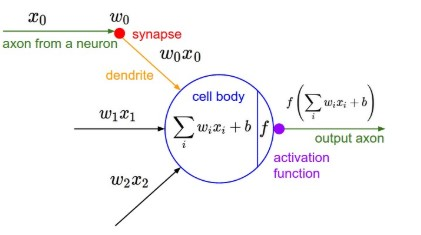
\includegraphics[width=0.70\textwidth]{CHAPTERS/Chapter-3/Images/3_1.jpg}
	\caption{Working of a single computational node}
	\label{fig:3.1}
\end{figure}

These neurons or computational nodes are organized 
into layer where there are highly interconnected to the neurons 
of following layer. The input layer of the feed forward neural 
networks feeds the information to the network and no kind of mathematical 
computation is performed. The hidden layer also known as distillation layer 
acts like a cell body and performs computation to extract salient features and 
patterns from the input data. A simple feed forward neural network with one 
hidden layer is shown in \ref{fig:3.2} \cite{chap_3_article:2}.
The output layer simply provides the results for given information. 

\begin{figure}[H]
	\centering
		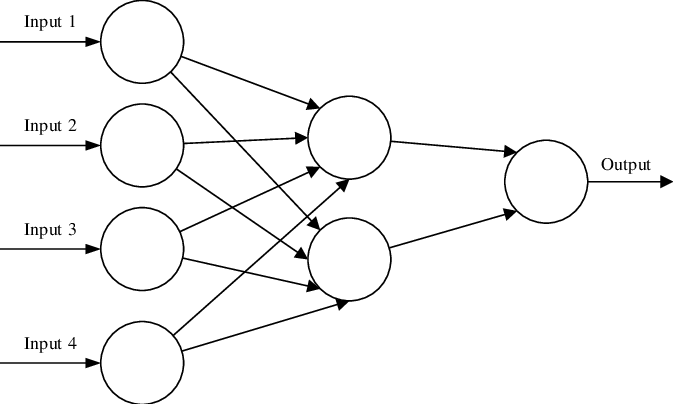
\includegraphics[width=0.70\textwidth]{CHAPTERS/Chapter-3/Images/3.2.png}
	\caption{Simple Feed Forward Neural Network with one hidden layer}
	\label{fig:3.2}
\end{figure}

The pixels of the image are arranged in a particular 
manner i.e. the appearance of the picture will be changed 
if we change the coordinate of one pixel. However, simple feed 
forward neural network loses to learn the inherent spatial 
relationships within images and fails to extract high level features 
needed for image classification. CNNs are types 
of neural networks that learn visual filters to recognize higher level 
image features and the spatial information is preserved. As a result, you 
end up learning this hierarchy of filters where filters at the early stage 
usually represents low level features like edge detection, gradient orientation 
and learning more and more complex features in the later stages.

\section{Convolutional Neural Networks Architecture}

CNNs consist of three types of layers. These layers 
include convolutional layers, pooling layers and fully connected layers. When 
these layers are stacked together, we get a CNN architecture. A general
architecture of CNNs with two convolutional layers is shown in \ref{fig:3.3} \cite{chap_3_article:2}.

\begin{figure}[H]
	\centering
		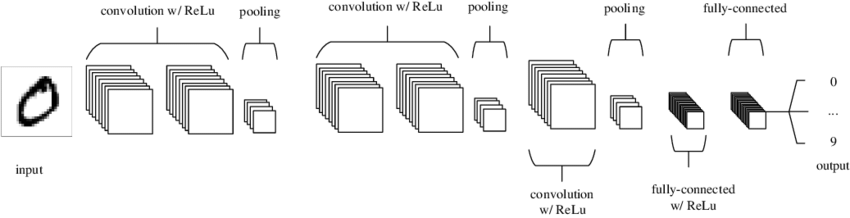
\includegraphics[width=0.80\textwidth]{CHAPTERS/Chapter-3/Images/3.3}
	\caption{Convolutional Neural Network Architecture with two convolutional layers}
	\label{fig:3.3}
\end{figure}

\subsection{Convolutional Layer}
Convolutional layers are integral part of CNNs and when these layers are stacked
 together, we start extracting more simple 
features and then aggregating these into more complex features later 
on. It consists of the set of learnable filters also known as kernels whose
height and width are smaller than the input image and always extend 
to the full depth of the input volume. We slide the filter over entire 
image to perform the mathematical operation of convolution i.e. element-wise 
multiplication of input image with the feature detector. The resultants are 
summed up and the value is assigned to the top left corner of receptive field 
as shown in figure 3.4 \cite{chap_3_article:4}.

\begin{figure}[H]
	\centering
		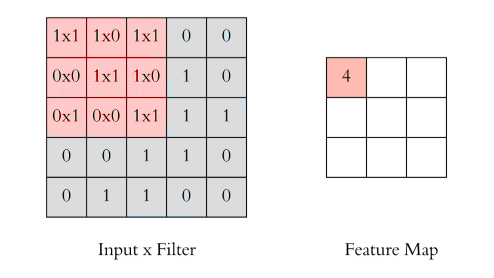
\includegraphics[width=0.70\textwidth]{CHAPTERS/Chapter-3/Images/3.4}
	\caption{3x3 filter with stride value of 1}
	\label{fig:3.4}
\end{figure}

The kernel window slides right or downward by a 
certain value in each step called the stride value and 
the process is repeated until the entire image is processed. Stride value of
1 moves the filter 1 pixel in each step. This results in a feature map with 
much smaller size than the input image and keeps on shrinking at every layer 
which is usually not desirable. Thus, dimensionality of the input image can be 
preserved by padding zero-pixel values across every side of image.

\begin{figure}[H]
	\centering
		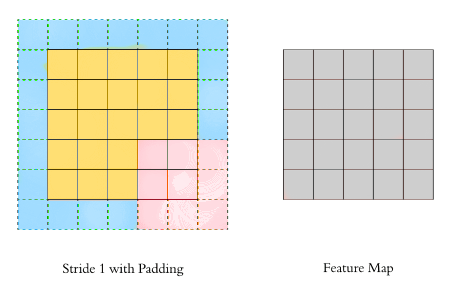
\includegraphics[width=0.70\textwidth]{CHAPTERS/Chapter-3/Images/3.5}
	\caption{Result  of 3x3 filter of Stride 1 with padding}
	\label{fig:3.5}
\end{figure}

In reality, we apply multiple filters to the same 
input image and feature maps are obtained depending upon the 
number of filters. In this case the output of convolutional layer 
is represented with a 3D matrix with dimensions of height, width 
and depth, where depth 
shows the no. of filters applied on the image. 

\begin{figure}[H]
	\centering
		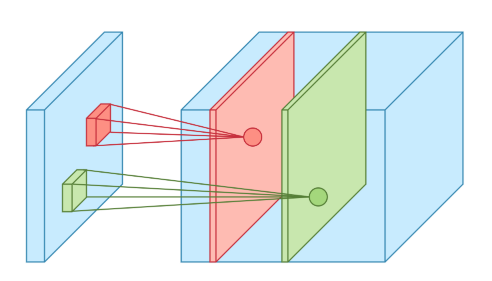
\includegraphics[width=0.70\textwidth]{CHAPTERS/Chapter-3/Images/3.6}
	\caption{Multiple filters applied on one input}
	\label{fig:3.6}
\end{figure}

\subsubsection{Activation Functions}

It is a mathematical function that is applied to every neuron 
in the network and decides whether a neuron should be activated 
or not depending on how much neuron’s input is relevant to model’s prediction. 
The main purpose of the activation function is to introduce non-linearity in the 
output. Without activation function, our network will be reduced to a simple 
regression model which would be unable to model and learn complex and complicated 
form of data. Thus, non-linear functions make neural networks capable 
of performing non-linear transformations to learn complex kinds of data such 
as 	images, videos etc. A good activation 
function should have the following properties:
\begin{itemize}
\item It should be zero centered because when back propagating gradient descent, the resulting values of gradient will either be all positive or all negative. Thus, it will affect the gradient based optimization process as we can only follow zig-zag path to reach the optimal point.
\item It shouldn’t kill the gradient flow i.e. neurons get saturated on the boundaries of activation and local gradient comes out to be zero. As a result, it nullifies the gradient flow during back propagation and dead neurons will stop updating.
\item It should be computationally efficient as activation function will be computed across millions of neurons for each input. Moreover, back propagation technique also puts constraint on the choice of activation function i.e. it should be differentiable.

\end{itemize}

\paragraph*{Sigmoid Function:}
A sigmoid function can be represented by the mathematical function:
\begin{equation}
	sig(z) = \frac{1}{1+e^{-z}}
\end{equation}
This function takes a real value as an input and squeezes 
it between 0 and -1 i.e. very large values. It is often known 
as squashing function as the large negative and positive 
values becomes 0 and 1 respectively \cite{chap_3_article:5} . However, the sigmoid function 
output is not zero-centered, and it also kills the neurons as function 
gets saturated at higher values. That’s why sigmoid function are usually 
not preferred in neural networks because of these drawbacks.

\begin{figure}[H]
	\centering
		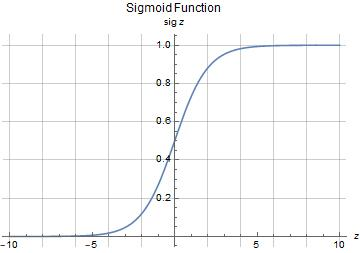
\includegraphics[width=0.70\textwidth]{CHAPTERS/Chapter-3/Images/3.7.jpg}
	\caption{Sigmoid Function}
	\label{fig:3.7}
\end{figure}
\paragraph*{Tanh Function:}
A tanh sigmoid function can be represented by the following mathematical function:
\begin{equation}
	tanh(z) = \frac{e^{z}-e^{-z}}{e^{z}+e^{-z}}
\end{equation}

It takes the real input value and squashed it between -1 and 1 i.e. very 
large negative and positive values are mapped into -1 and 1 respectively \cite{chap_3_article:5}. As 
a result, this non-linear activation function gives zero-mean data, but it 
still gets saturated at higher values as shown in \ref{fig:3.8}. However, tanh 
activations functions are preferred over sigmoid functions in neural networks.

\begin{figure}[H]
	\centering
		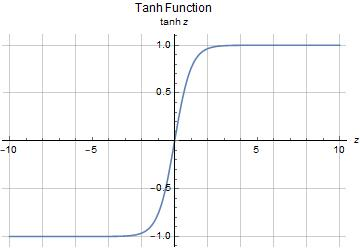
\includegraphics[width=0.70\textwidth]{CHAPTERS/Chapter-3/Images/3.8.jpg}
	\caption{Tanh function}
	\label{fig:3.8}
\end{figure}

\paragraph*{ReLU Function:}
ReLU stands for Rectified Linear unit and is represented by the following equation:

\begin{equation}
	ReLU(z) = max(0,z)
\end{equation}

It takes real values as an input and sets all the negative 
values equal to zero \cite{chap_3_article:3}. It is computationally very efficient as no 
complicated math need to be performed. And it is the most commonly used 
activation function in neural networks as it increases the convergence rate 
of gradient descent by six times as compared to sigmoid and tanh activation 
functions. However, the function doesn’t get saturated for larger values of 
inputs, but the neurons often stuck in a negative side giving zero local gradient 
and neuron will never get a chance to update in gradient descent learning process. 
This problem is also known as dying ReLU and it often occurs due to high learning 
rate or there is a large negative bias. Leaky ReLU can be used to avoid this 
situation. Leaky ReLU is very similar to original ReLU and the only difference 
is that now instead of being flat in the negative regime, we are going to give 
slight negative slope here. This solves a lot of problems we mentioned earlier
as it doesn’t saturate in the negative space and still very computationally efficient \cite{chap_3_article:3}.

% \begin{figure}
% 	\centering
% 	\begin{subfigure}{.5\textwidth}
% 	  \centering
% 	  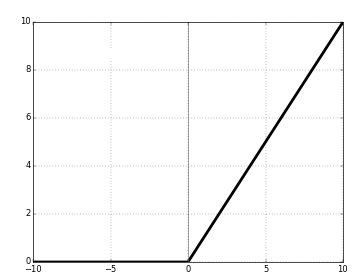
\includegraphics[width=.4\linewidth]{CHAPTERS/Chapter-3/Images/3.9a}
% 	  \caption{A subfigure}
% 	  \label{fig:3.9(a)}
% 	\end{subfigure}%
% 	\begin{subfigure}{.5\textwidth}
% 	  \centering
% 	  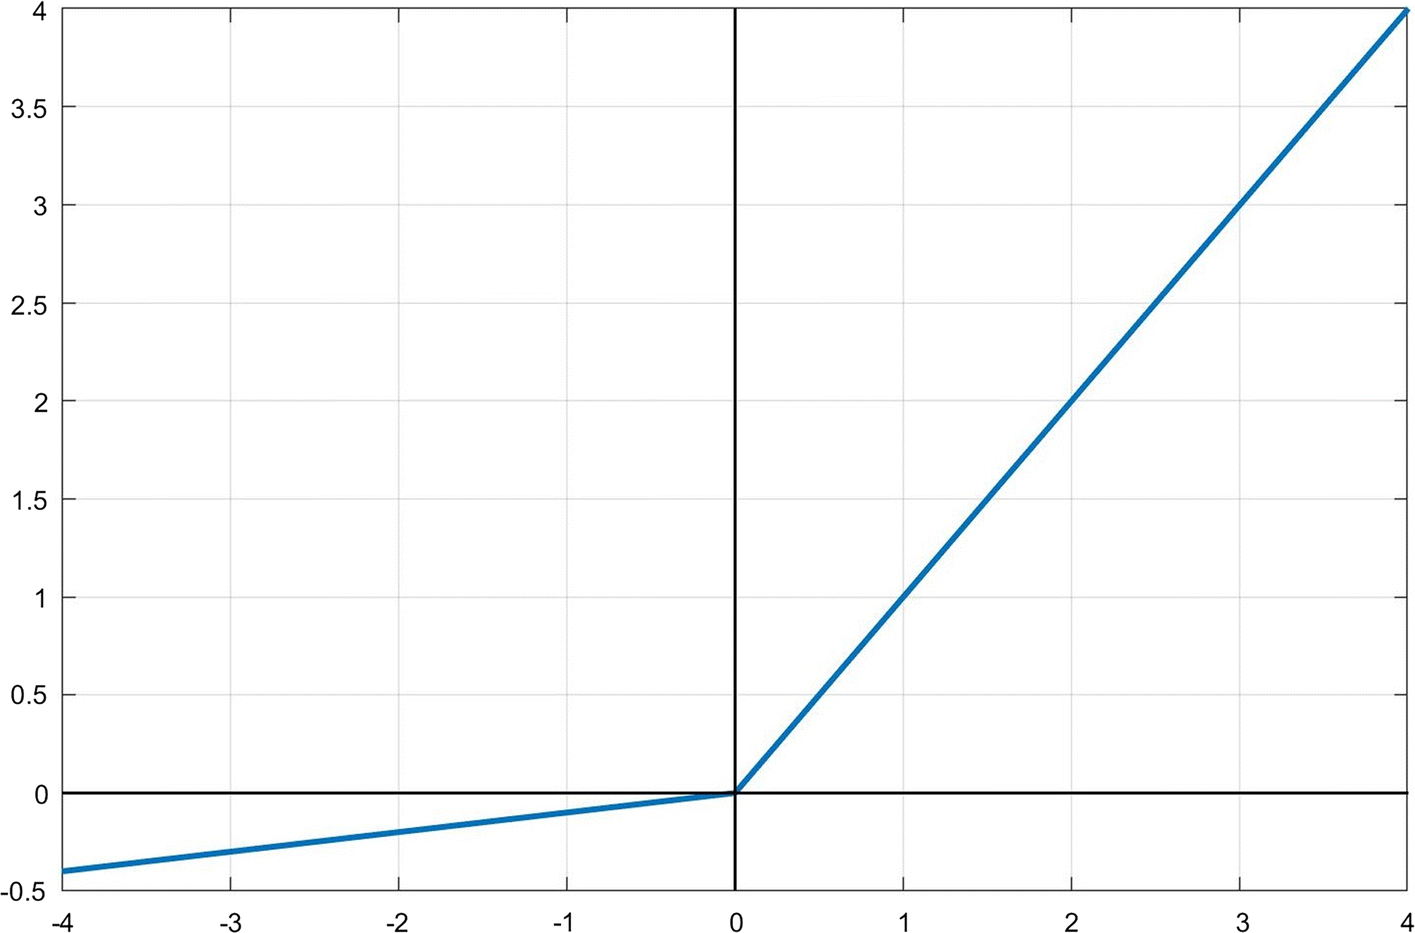
\includegraphics[width=.4\linewidth]{CHAPTERS/Chapter-3/Images/3.9b}
% 	  \caption{A subfigure}
% 	  \label{fig:3.9(b)}
% 	\end{subfigure}
% 	\caption{ReLU and Leaky ReLU Function}
% 	\label{fig:test}
% \end{figure}

\begin{figure}%
    \centering
    \subfloat[\label{fig:3.9(a)}]{{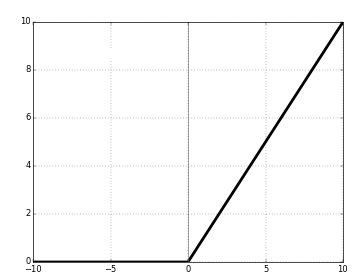
\includegraphics[height = 4.38cm, width=5cm]{CHAPTERS/Chapter-3/Images/3.9a} }}%
    \qquad
    \subfloat[\label{fig:3.9(b)}]{{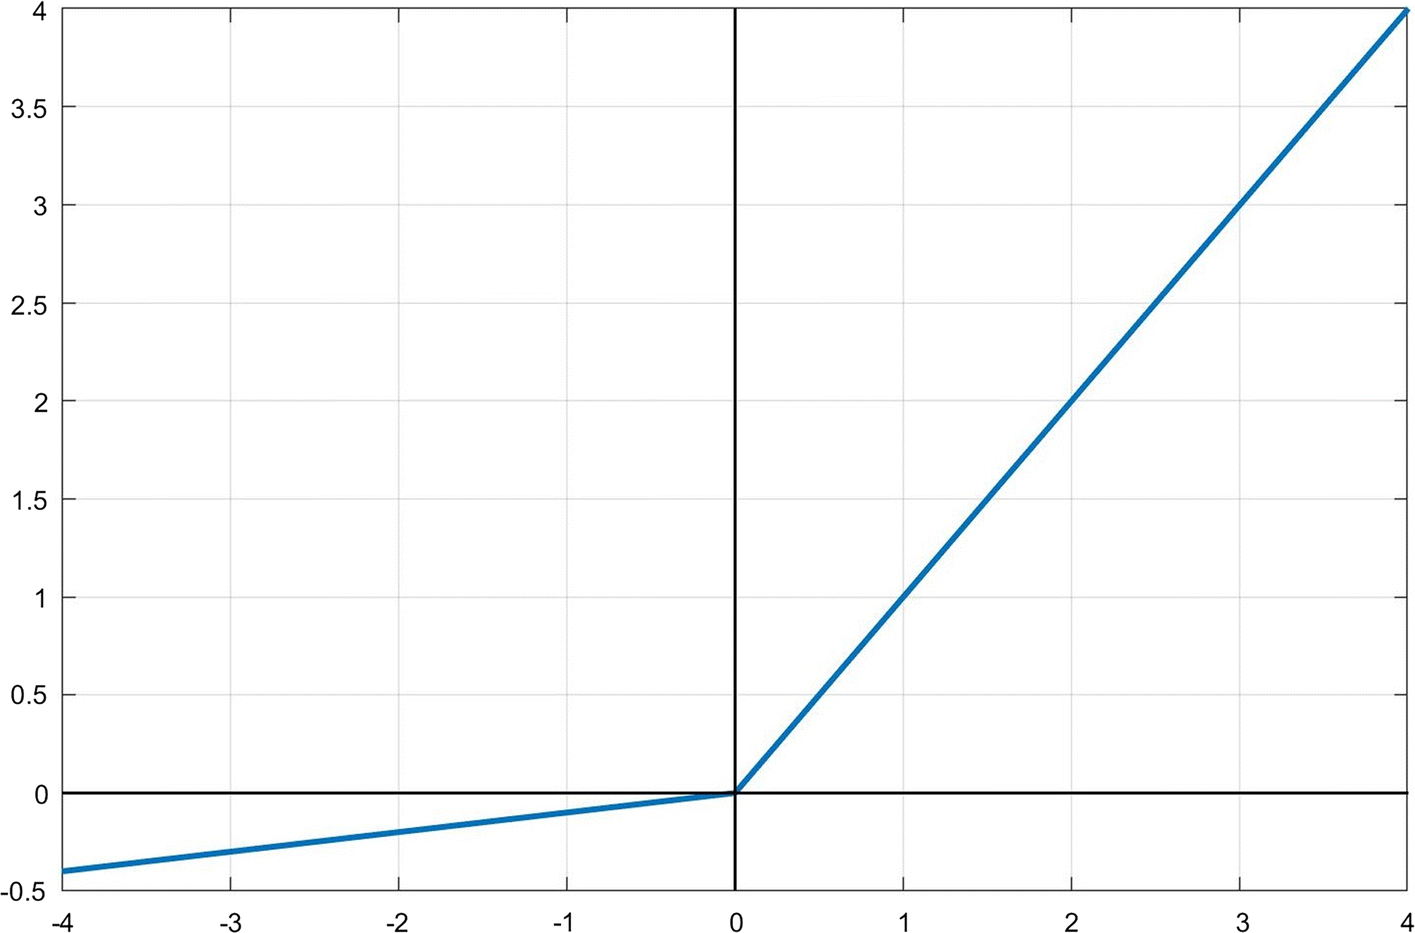
\includegraphics[height = 4cm, width=5cm]{CHAPTERS/Chapter-3/Images/3.9b} }}%
    \caption{ReLU and Leaky ReLU Function}%
    \label{fig:3.9}%
\end{figure}

\subsection{Pooling Layer}
Pooling layer follows the non-linear function introduced in convolutional layer 
in CNN. It simply down samples the feature map to 
speed up the computation as well as make some of the features it detects a bit 
more robust \cite{chap_3_article:4}. Rest of the operations will be performed on the summarized features so that the feature map is no more sensitive to the
 precise location of features in the input. Two most 
commonly used pooling techniques are described below:

\subsubsection{Average Pooling}

In average pooling, we simply place the filter window and 
find the average of pixel values covered by the filter on 
the feature map. We simply keep on sliding the filter and repeat 
the process until entire input image is processed. The average pooling 
technique with 2 x 2 filter size and 
stride value of 2 is illustrated in \ref{fig:3.10(a)}.

\subsubsection{Max Pooling}
It is a pooling technique in which the most prominent 
features in the region of feature map are retained. We simply 
take the maximum value present under filter and process the entire 
feature map to get a down-sampled output as shown in \ref{fig:3.10(b)} \cite{chap_3_article:6}.

\begin{figure}%
    \centering
    \subfloat[\label{fig:3.10(a)}]{{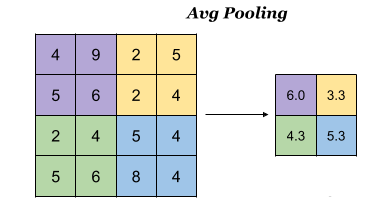
\includegraphics[height = 4cm, width=6cm]{CHAPTERS/Chapter-3/Images/3.10a} }}%
    \qquad
    \subfloat[\label{fig:3.10(b)}]{{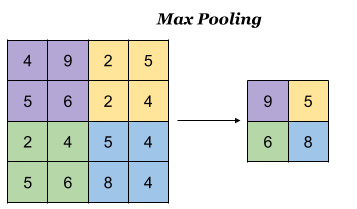
\includegraphics[height = 4cm, width=6cm]{CHAPTERS/Chapter-3/Images/3.10b} }}%
    \caption{Average and Max Pooling}%
    \label{fig:3.10}%
\end{figure}

\subsection{Flatten Layer}

The flatter layer acts as bridge between last convolutional or pooling layer 
and fully connected layer. The function of the flatten layer is to simply take
a two-dimensional feature map and stretch it into a long column vector that acts as 
an input to the fully connected layer of artificial neural network.


\begin{figure}[H]
	\centering
		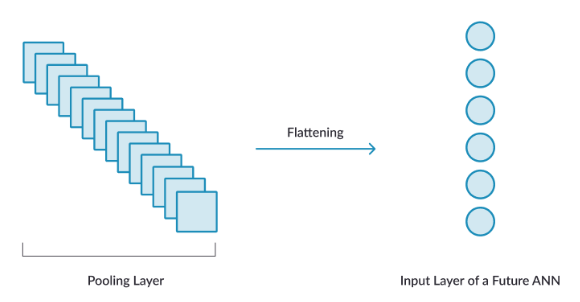
\includegraphics[width=0.60\textwidth]{CHAPTERS/Chapter-3/Images/3.11}
	\caption{Flatten layer}
	\label{fig:3.11}
\end{figure}


\subsection{Fully Connected Layer} 

Fully connected layer is considered as an important 
part of CNNs and gives the final 
probabilities for each class.  The output feature value vector obtained by the flatting layer is 
given as input to the fully connected layer. It classifies the input image into various classes using these features. The output is simply a vector 
of m $\times$ 1 dimension giving the probability of the 
classification label model is trying to predict. The probabilities of the
classes are obtained using Softman activation function which simply squashes the input values between 0 and 1 that sums to one.

Thus we conclude that CNNs are divided into two separate categories i.e. feature learning and classification. In feature learning part,
 data is passed through convolutional layer, activation functioin and pooling layer over and over again to extract several types
of features from the images. The resulting feature matrix is passed to classification
layer where it is flattened to a single vector and get probability for each class as an output of fully connected layer.